\chapter{GPU, CUDA}
Le GPU (Graphics Processing Units) emergono alla fine degli anni '90 come hardware specializzato per il rendering grafico 3D, in risposta a una necessità critica: la CPU non era in grado di gestire in modo efficiente il carico computazionale richiesto dalle applicazioni grafiche real-time (videogiochi, animazioni, simulazioni visive).
Nel 1999, NVIDIA rilascia sul mercato la GeForce 256, pubblicizzandola per la prima volta come \q{GPU}, sottolineando la sua capacità di accelerare le operazioni grafiche senza coinvolgere la CPU. 
Per l'HPC, il vero salto avviene con l'introduzione delle GPGPU (General-Purpose GPU), che trasformano le GPU da acceleratori grafici a processori paralleli universali.
Nel 2006, NVIDIA lancia CUDA (Compute Unified Device Architecture), un framework C/C++ per la programmazione parallela su GPU, dando definitivamente il via all'utilizzo general purpose delle GPU. 
Nel 2007, AMD risponde con il lancio del framework ATI Stream\footnote{Ad oggi, AMD sviluppa il framework proprietario ROCm}. 
Tuttavia, sia CUDA che ATI Stream erano framework proprietari e per giunta funzionanti solo sulle GPU di, rispettivamente, NVIDIA e AMD.
Con lo scopo di definire un framework interoperabile, nel 2009, Khronos Group rilascia la specifica OpenCL.
Tuttavia, NVIDIA depreca OpenCL nel 2017 e AMD sposta la sua attenzione su ROCm a partire dal 2016. 
Allora, il Khronos Group rilascia, nel 2018, una nuova specifica, SYCL, inizialmente nata come estensione di OpenCL, che permette di unificare il codice per CPU e GPU in modo più naturale rispetto ai framework precedenti e che sta trovando crescente supporto da parte dei principali produttori hardware, tra cui NVIDIA (con DPC++), AMD (con hipSYCL), e Intel (con Intel oneAPI), che stanno adottando SYCL come standard per il calcolo parallelo moderno.
Allo stato attuale, però, CUDA garantisce ancora le migliori performance su hardware NVIDIA, grazie a decenni di ottimizzazioni e a un ecosistema maturo.

\begin{note}{Terminologia}
Una GPU è comunemente chiamata \keyword{acceleratore} o \keyword{device} poiché comunemente utilizzata per accelerare calcoli \q{molto paralleli} che la CPU soddisferebbe in modo poco efficiente.
\end{note}

\section{Architettura CUDA}
CUDA è un'architettura ibrida che presenta tre livelli di parallelismo. Il primo, macroscopico, prevede la presenza di $p$ \keyword{Streaming Multiprocessor} (SM), che condividono tra loro la \keyword{global memory}. Quindi, a questo livello macroscopico, l'architettura è MIMD Shared Memory. Il secondo livello, intermedio, prevede che ciascun SM sia un calcolatore SIMD dotato di $Q$ \keyword{CUDA cores}. Ciascun SM ha una memoria condivisa, detta \keyword{shared memory}, a cui possono accedere i CUDA cores. Ciascun CUDA core è dotato di una memoria locale e privata. Ciascun SM, essendo SIMD, gestisce un tipo di operazione alla volta, poiché ha una sola unità di controllo.

\begin{observation}{}
Nella classica architettura SIMD, un \texttt{if-else} viene eseguito in modo sequenziale: il primo ramo viene eseguito da tutte le ALU che devono eseguire tale ramo, mentre le altre ALU aspettano; il secondo ramo viene eseguito dopo il primo dalle ALU che devono eseguire tale ramo, mentre le altre ALU aspettano. 
Ciascuno dei $Q$ CUDA cores è in realtà un processore minimale con capacità di branching, che, in presenza di un \texttt{if-else}, consente l'esecuzione simultanea dei due rami, senza che nessun CUDA core debba aspettare.
La capacità di branching, di fatto, permette di eseguire in modo indipendente un thread, a patto che il codice da eseguire sia identico al codice gestito dall'unità di controllo dell'SM di cui fa parte.
Infatti, ciascun SM è detto SIMT (Single Instruction stream Multiple Threads).
\end{observation}

L'ultimo livello di parallelismo prevede che ciascun CUDA core implementi una pipeline. La CU di un SM impiega $k$ cicli macchina per la decodifica di un'operazione, mentre un CUDA core solo $1$. Definiamo $r$ il numero di cicli necessari alla pipeline di un CUDA core per andare a regime.

\begin{note}{}
Si assume $k<r$, altrimenti la pipeline di un CUDA core non potrebbe mai andare a regime.
\end{note}

In questa situazione, invece di far eseguire ad un CUDA core una sola operazione per $k$ cicli, la stessa operazione, ovviamente su dati diversi, viene eseguita $k$ volte, da $k$ thread diversi. Quindi, su ciascun CUDA core è possibile eseguire $k$ thread. Poiché un SM ha $Q$ CUDA cores, su ciascun SM è possibile eseguire $k\cdot Q=:\dim W$ thread, dove $W$, detto \keyword{warp}, è l'insieme dei thread che eseguono in parallelo su un singolo SM. L'intera macchina possiede $p$ processori SM, per cui essa può eseguire contemporaneamente $p\cdot \dim W$ thread.

\begin{note}{}
Il valore $\dim W$ è, di fatto, il minimo numero di thread che ha senso lanciare su un processore SM per sfruttare il suo parallelismo. Essendo un processore SM una macchina SIMD, anche lanciando meno thread, essa comunque farà uso di tutti i suoi CUDA cores. Pertanto, lanciando meno di $\dim W$ thread, non solo non si sfrutterà appieno il parallelismo, ma non sarà possibile nemmeno risparmiare energia.
\end{note}


\begin{figure}[h]
\centering
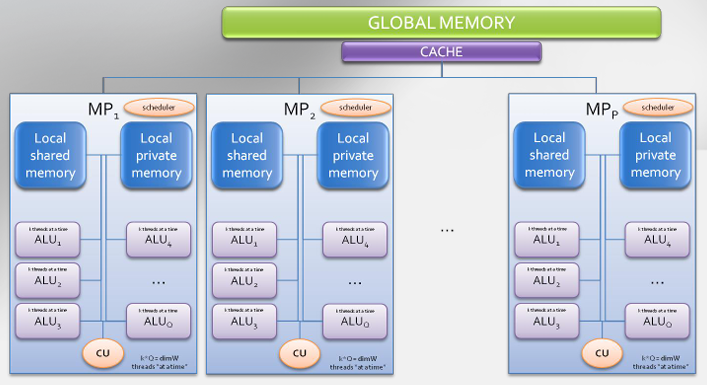
\includegraphics[width=0.8\textwidth]{../_files/_images/cuda-arch.png}
\caption{Lo schema architetturale CUDA, ricavato dal white paper di NVIDIA e confermato da test empirici. Gli MP corrispondono ai SM, mentre le ALU corrispondono ai CUDA cores. Ciascun CUDA core possiede una "Local private memory".}
\label{fig:cuda-arch}
\end{figure}

Quindi, il tempo di esecuzione ideale di una GPU su un problema di dimensione $n$ è 
$$T_{GPU}(n)= \frac{T(n)}{p\cdot \dim W} t_{calc}$$
dove $T(n)$ è il numero di operazione per risolvere il problema di dimensione $n$ e $t_{calc}$ è il tempo per eseguire una floating point operation (flop).
Idealmente, si dovrebbe avere $S_{\text{GPU}}(n)=\frac{T(n)}{T_{\text{GPU}}(n)}=p\cdot\dim W$. Tuttavia, a $T_{\text{GPU}}(n)$ va aggiunto il tempo di accesso alla memoria, $T_{mem}(n)$, che è capace di far degradare lo speedup. Però, aumentando sia il numero di thread che la dimensione del problema, si osserva che $T_{mem}$ impatta sempre di meno sul tempo di esecuzione totale, $T_{\text{GPU}}$, portando a speedup migliori. Questa strategia per ridurre l'overhead è analoga a quella vista per l'overhead di comunicazione nel precedente capitolo.
Con le GPU, si ragiona tipicamente per scalabilità debole.

\section{Programmazione CUDA}
All'architettura descritta finora corrisponde un framework di programmazione, CUDA C/C++, costruito come estensione dei linguaggi C e C++ ed ideato per la scrittura di programmi eseguibili in ambienti eterogenei, ovvero in presenza di CPU e GPU.
La CPU tiene le redini del flusso logico del programma e, quando opportuno, fa uso della GPU come acceleratore.
Per questo motivo, la CPU è chiamata \keyword{host} e la GPU, invece, \keyword{device}.

\subsection{Concetti}
Nel framework CUDA, si lavora con un'astrazione dell'architettura descritta nella sezione precedente: ciascun CUDA core esegue un \keyword{thread}, ciascun SM esegue un \keyword{thread block} (blocco), ovvero un gruppo di thread, e l'intera GPU esegue una \keyword{grid} (griglia), ovvero un gruppo di blocchi.
Sia una griglia che un blocco sono tensori tridimensionali.
Ciò permette di definire una topologia secondo lo schema scelto per la suddivisione del calcolo.
All'interno di una griglia, tutti i blocchi devono avere la stessa forma, ovvero le stesse dimensioni, per consentire l'indirizzamento a tempo costante e memoria zero.\footnote{Altrimenti, bisognerebbe conservare, per ogni blocco, la sua forma, ed effettuare calcoli complessi per ricavare un indice globale per ciascun thread.}
I thread all'interno di ciascun blocco sono raggruppati in \keyword{warp}.
La dimensione di un warp è stabilmente \(32\) dalla Compute Capability \(1.0\)\footnote{La Compute Capability è un numero di versione che indica le caratteristiche, le specifiche e l'instruction set supportato da una specifica architettura CUDA. Conoscere la Compute Capability del device a disposizione è cruciale per l'ottimizzazione degli algoritmi su di esso.}.
I thread di un warp eseguono in \keyword{lockstep}\footnote{In realtà, a partire dalla Compute Capability \(7.0\), ciò non è più vero. È possibile, in tali device, lo scheduling asincrono di thread dello stesso warp.}, ovvero eseguono in modo sincronizzato, secondo la specifica SIMT, di cui abbiamo precedentemente parlato.

\begin{observation}{Curiosità}
    La traduzione di \textit{thread} in italiano è \textit{filo}, mentre quella di \textit{warp} è \textit{ordito}, ossia l'insieme dei fili tesi sul telaio che si intrecciano con la trama.
\end{observation}

\subsection{Kernel, funzioni}
Un \keyword{kernel} è una funzione invocata dall'host ed eseguita sul device. Un kernel è eseguito da una griglia di thread. Tutti i thread della griglia eseguono il kernel.
Un kernel è una funzione \texttt{void}, con scope \texttt{\_\_global\_\_}.

\begin{lstlisting}[language=C++, numbers=none]
__global__ void kernel_name(arguments) {
    // Kernel code executed by each thread.
}
\end{lstlisting}

In CUDA, ogni funzione ha uno scope in termini di invocazione ed esecuzione rispetto a host e device.
Una funzione \texttt{\_\_global} può essere invocata solo dall'host ed eseguita sul device.
Una funzione \texttt{\_\_device\_\_} può essere invocata solo dal device ed eseguita sul device.
Una funzione \texttt{\_\_host\_\_} può essere invocata solo dall'host ed eseguita sull'host.
Se non specificato, lo scope di una funzione è \texttt{\_\_host\_\_}.
Una funzione \texttt{\_\_host\_\_ \_\_device\_\_} può essere invocata sia dall'host che dal device e può eseguire su entrambi.

\begin{note}{}
    Nelle funzioni eseguibili su device, sono proibite la ricorsione, le variabili statiche, numero variabile di argomenti (funzioni variadiche).
\end{note}

Un kernel viene invocato dall'host specificando due parametri obbligatori (i primi) e due opzionali (gli ultimi).

\begin{lstlisting}[language=C++, numbers=none]
kernel_name<<<dim_grid, dim_block, shared_mem_size, stream>>>(arguments);
\end{lstlisting}

Per ora, ci concentreremo sui primi due: \texttt{dim\_grid} è la forma della griglia da eseguire, \texttt{dim\_block} è la forma di ciascun blocco.

\subsection{Memoria}
Per comprendere la programmazione CUDA, risulta cruciale interessarsi della gerarchia di memorie che l'architettura offre. 
Come vedremo tra poco, vi è un mapping uno a uno tra la memoria descritta durante la presentazione dell'architettura CUDA e la memoria accessibile in un programma CUDA.

\subsubsection{Memoria centrale}
In CUDA, la memoria centrale dell'host e la global memory della GPU sono separate: è richiesto un trasferimento esplicito di dati tra le due.
Di conseguenza, separata è anche l'allocazione delle due memorie.
La memoria centrale dell'host è allocabile secondo le stesse modalità che i linguaggi C e C++ offrono, mentre la global memory richiede funzioni proprie del framework CUDA.
Così come per la memoria centrale, l'allocazione della global memory può avvenire sia staticamente che dinamicamente.
Una variabile allocata staticamente dev'essere dichiarata al di fuori di qualsiasi funzione e con la keyword \texttt{\_\_device\_\_}, omonima di quella applicata a funzioni.

\begin{lstlisting}[language=C++, numbers=none]
__device__ float array[1024];
\end{lstlisting}

Una variabile può essere allocata dinamicamente mediante le funzioni di allocazione di CUDA, di cui \texttt{cudaMalloc} è la più semplice.

\begin{lstlisting}[language=C++, numbers=none]
/*
 * cudaError_t cudaMalloc(void **devPtr, size_t size)	
 * 
 * Parameters:
 *  devPtr: pointer to allocated device memory
 *  size: requested allocation size in bytes
 *
 * Returns:
 *  cudaSuccess, cudaErrorMemoryAllocation
 */

float *array = NULL; 
const uint size = 1024;
cudaMalloc((void **) &array, size * sizeof(float));
//[...]
cudaFree(array);
array = NULL;
\end{lstlisting}

%TODO: trasferimento da memoria centrale a global memory e viceversa
Tipicamente, un kernel viene invocato per il calcolo di uno o più valori.
Poiché un kernel è una funzione \texttt{void}, è necessario passare al kernel un puntatore alla variabile, che risiede sulla global memory, che conterrà il risultato.
Per elaborare il risultato sull'host, occorre effettuare un trasferimento del dato dalla global memory alla memoria centrale dell'host.
Il metodo di base per farlo è mediante la funzione \texttt{cudaMemcpy}.

\begin{lstlisting}[language=C++, numbers=none]
/*
 * __host__ cudaError_t cudaMemcpy(
 *      void *dst, const void *src, size_t count,
 *      cudaMemcpyKind kind
 * )
 * 
 * Parameters:
 *  dst: destination memory address
 *  src: source memory address
 *  count: size in bytes to copy
 *  kind: type of transfer:
 *      cudaMemcpyHostToHost, cudaMemcpyHostToDevice,
 *      cudaMemcpyDeviceToHost, cudaMemcpyDeviceToDevice,
 *      cudaMemcpyDefault (for UnifiedMemory, we'll see it)
 *
 * Returns:
 *  cudaSuccess, cudaErrorInvalidValue,
 *  cudaErrorInvalidMemcpyDirection
 */

float *result, *result_dev;
//[...]
some_kernel<<<dim_grid, dim_block>>>(result_dev);
//[...]
cudaMemcpy(
    result, result_dev, sizeof(float) * size,
    cudaMemcpyDeviceToHost
);
\end{lstlisting}

\begin{observation}{Unified Memory}
%TODO: approfondimento
Per device con Compute Capability \(\geq 6.0\), è possibile l'utilizzo della \keyword{unified memory}, ossia una memoria virtuale che unifica, appunto, la global memory con la memoria centrale dell'host.
È possibile allocare una variabile in unified memory mediante la funzione \texttt{cudaMallocManaged}, che permette di allocare memoria accessibile sia dall'host che dal device.
In questo modo, non è necessario un trasferimento esplicito dei dati, poiché è la unified memory a spostare i dati quando richiesto.
\end{observation}

\subsubsection{Shared memory}
Nella programmazione CUDA, l'utilizzo della global memory andrebbe limitato al massimo, data la presenza di memorie molto più veloci, ovvero la shared memory e i registri dei CUDA cores.
I thread all'interno dello stesso blocco possono accedere alla shared memory, che è generalmente di un ordine di grandezza più veloce della global memory per accesso e scrittura.
È possibile allocare memoria sulla shared memory sia staticamente che dinamicamente.
Per allocare una variabile in modo statico, è possibile dichiararla, all'interno del kernel, con la keyword \texttt{\_\_shared\_\_}.

\begin{lstlisting}[language=C++, numbers=none]
__shared__ float shared_data[1024];
\end{lstlisting}

Per allocare una variabile in modo dinamico, è necessario specificare la dimensione in byte della shared memory da allocare come terzo parametro di lancio del kernel.
All'interno del kernel, è necessario dichiarare la variabile con \texttt{extern}, oltre che con \texttt{\_\_shared\_\_}, senza specificare la sua dimensione, che sarà stabilita a run time.

\begin{lstlisting}[language=C++, numbers=none]
//Inside invoker
some_kernel<<<dim_grid, dim_block, shared_mem_size>>>(arguments);

//Inside kernel
extern __shared__ shared_data[];
\end{lstlisting}

\begin{note}{}
    \texttt{shared\_mem\_size} corrisponde alla dimensione della shared memory da allocare per tutti i blocchi.
    Ad esempio, se vogliamo che ogni blocco abbia a disposizione \texttt{size} byte, allora \texttt{shared\_mem\_size} dovrà essere uguale a \texttt{size} moltiplicato per il numero di blocchi.
\end{note}

%TODO: Cita https://feldmann.nyc/blog/smem-microbenchmarks
Per consentire l'uso efficiente della shared memory da parte dei thread di un warp, essa è suddivisa in \(32\) \keyword{banchi} (o, banks).
Ogni banco è una porzione di shared memory di \(4\) byte.
Ciascun banco può effettuare lettura e scrittura in un singolo ciclo macchina.
La suddivisione in banchi è circolare: premettendo che la shared memory è \textit{byte-addressed}\footnote{Una memoria è byte-addressed quando presenta un indirizzo di memoria per ogni suo byte.}, i suoi indirizzi sono suddivisi in banchi secondo la funzione \texttt{bank(addr) = (addr/4) \% 32}.
Ciò significa che, dato un array in shared memory \texttt{\_\_shared\_\_ float s[64]}, gli elementi \texttt{s[0]}, \texttt{s[32]} appartengono allo stesso banco, gli elementi \texttt{s[1]}, \texttt{s[33]} appartengono al banco successivo e così via.

Accessi allo stesso banco vengono serializzati, mentre accessi a banchi diversi avvengono simultaneamente.
Se tutti i thread devono leggere dallo stesso indirizzo dello stesso banco, allora il valore contenuto in tale indirizzo viene trasmesso simultaneamente ai thread richiedenti. Questa proprietà è chiamata \keyword{broadcasting}.
Inoltre, la shared memory consente anche il \keyword{multicasting}, che consente più broadcasting simultanei.
Ad esempio, sempre all'interno dello stesso warp, se un gruppo di thread, \(G_{1}\), vuole leggere il valore \texttt{s[0]} e un altro gruppo di thread, \(G_{2}\), vuole leggere il valore \texttt{s[1]}, allora \texttt{s[0]} viene trasmesso simultaneamente a tutti i thread di \(G_{1}\) e \texttt{s[1]} viene trasmesso simultaneamente a tutti i thread di \(G_{2}\).
